\documentclass[9pt]{beamer}

% Beamer style
%\usetheme[secheader]{Madrid}
% \usetheme{CambridgeUS}
\useoutertheme{infolines}
\usecolortheme[rgb={0.65,0.15,0.25}]{structure}
% \usefonttheme[onlymath]{serif}
\beamertemplatenavigationsymbolsempty
%\AtBeginSubsection

% Packages
%\usepackage[french]{babel}
\usepackage[latin1]{inputenc}
\usepackage{color}
\usepackage{xspace}
\usepackage{dsfont, stmaryrd}
\usepackage{amsmath, amsfonts, amssymb, stmaryrd}
\usepackage{epsfig}
\usepackage{tikz}
\usepackage{url}
% \usepackage{ulem}
\usepackage{/home/robin/LATEX/Biblio/astats}
%\usepackage[all]{xy}
\usepackage{graphicx}
\usepackage{xspace}

% Maths
% \newtheorem{theorem}{Theorem}
% \newtheorem{definition}{Definition}
\newtheorem{proposition}{Proposition}
% \newtheorem{assumption}{Assumption}
% \newtheorem{algorithm}{Algorithm}
% \newtheorem{lemma}{Lemma}
% \newtheorem{remark}{Remark}
% \newtheorem{exercise}{Exercise}
% \newcommand{\propname}{Prop.}
% \newcommand{\proof}{\noindent{\sl Proof:}\quad}
% \newcommand{\eproof}{$\blacksquare$}

% \setcounter{secnumdepth}{3}
% \setcounter{tocdepth}{3}
\newcommand{\pref}[1]{\ref{#1} p.\pageref{#1}}
\newcommand{\qref}[1]{\eqref{#1} p.\pageref{#1}}

% Colors : http://latexcolor.com/
\definecolor{darkred}{rgb}{0.65,0.15,0.25}
\definecolor{darkgreen}{rgb}{0,0.4,0}
\definecolor{darkred}{rgb}{0.65,0.15,0.25}
\definecolor{amethyst}{rgb}{0.6, 0.4, 0.8}
\definecolor{asparagus}{rgb}{0.53, 0.66, 0.42}
\definecolor{applegreen}{rgb}{0.55, 0.71, 0.0}
\definecolor{awesome}{rgb}{1.0, 0.13, 0.32}
\definecolor{blue-green}{rgb}{0.0, 0.87, 0.87}
\definecolor{red-ggplot}{rgb}{0.52, 0.25, 0.23}
\definecolor{green-ggplot}{rgb}{0.42, 0.58, 0.00}
\definecolor{purple-ggplot}{rgb}{0.34, 0.21, 0.44}
\definecolor{blue-ggplot}{rgb}{0.00, 0.49, 0.51}

% Commands
\newcommand{\backupbegin}{
   \newcounter{finalframe}
   \setcounter{finalframe}{\value{framenumber}}
}
\newcommand{\backupend}{
   \setcounter{framenumber}{\value{finalframe}}
}
\newcommand{\emphase}[1]{\textcolor{darkred}{#1}}
\newcommand{\comment}[1]{\textcolor{gray}{#1}}
\newcommand{\paragraph}[1]{\textcolor{darkred}{#1}}
\newcommand{\refer}[1]{{\small{\textcolor{gray}{{\cite{#1}}}}}}
\newcommand{\Refer}[1]{{\small{\textcolor{gray}{{[#1]}}}}}
\newcommand{\goto}[1]{{\small{\textcolor{blue}{[\#\ref{#1}]}}}}
\renewcommand{\newblock}{}

\newcommand{\tabequation}[1]{{\medskip \centerline{#1} \medskip}}
% \renewcommand{\binom}[2]{{\left(\begin{array}{c} #1 \\ #2 \end{array}\right)}}

% Variables 
\newcommand{\Abf}{{\bf A}}
\newcommand{\Beta}{\text{B}}
\newcommand{\Bcal}{\mathcal{B}}
\newcommand{\Bias}{\xspace\mathbb B}
\newcommand{\Cor}{{\mathbb C}\text{or}}
\newcommand{\Cov}{{\mathbb C}\text{ov}}
\newcommand{\cl}{\text{\it c}\ell}
\newcommand{\Ccal}{\mathcal{C}}
\newcommand{\cst}{\text{cst}}
\newcommand{\Dcal}{\mathcal{D}}
\newcommand{\Ecal}{\mathcal{E}}
\newcommand{\Esp}{\xspace\mathbb E}
\newcommand{\Espt}{\widetilde{\Esp}}
\newcommand{\Covt}{\widetilde{\Cov}}
\newcommand{\Ibb}{\mathbb I}
\newcommand{\Fcal}{\mathcal{F}}
\newcommand{\Gcal}{\mathcal{G}}
\newcommand{\Gam}{\mathcal{G}\text{am}}
\newcommand{\Hcal}{\mathcal{H}}
\newcommand{\Jcal}{\mathcal{J}}
\newcommand{\Lcal}{\mathcal{L}}
\newcommand{\Mt}{\widetilde{M}}
\newcommand{\mt}{\widetilde{m}}
\newcommand{\Nbb}{\mathbb{N}}
\newcommand{\Mcal}{\mathcal{M}}
\newcommand{\Ncal}{\mathcal{N}}
\newcommand{\Ocal}{\mathcal{O}}
\newcommand{\pt}{\widetilde{p}}
\newcommand{\Pt}{\widetilde{P}}
\newcommand{\Pbb}{\mathbb{P}}
\newcommand{\Pcal}{\mathcal{P}}
\newcommand{\Qcal}{\mathcal{Q}}
\newcommand{\qt}{\widetilde{q}}
\newcommand{\Rbb}{\mathbb{R}}
\newcommand{\Sbb}{\mathbb{S}}
\newcommand{\Scal}{\mathcal{S}}
\newcommand{\st}{\widetilde{s}}
\newcommand{\St}{\widetilde{S}}
\newcommand{\Tcal}{\mathcal{T}}
\newcommand{\todo}{\textcolor{red}{TO DO}}
\newcommand{\Ucal}{\mathcal{U}}
\newcommand{\Un}{\math{1}}
\newcommand{\Vcal}{\mathcal{V}}
\newcommand{\Var}{\mathbb V}
\newcommand{\Vart}{\widetilde{\Var}}
\newcommand{\Zcal}{\mathcal{Z}}

% Symboles & notations
\newcommand\independent{\protect\mathpalette{\protect\independenT}{\perp}}\def\independenT#1#2{\mathrel{\rlap{$#1#2$}\mkern2mu{#1#2}}} 
\renewcommand{\d}{\text{\xspace d}}
\newcommand{\gv}{\mid}
\newcommand{\ggv}{\, \| \, }
% \newcommand{\diag}{\text{diag}}
\newcommand{\card}[1]{\text{card}\left(#1\right)}
\newcommand{\trace}[1]{\text{tr}\left(#1\right)}
\newcommand{\matr}[1]{\boldsymbol{#1}}
\newcommand{\matrbf}[1]{\mathbf{#1}}
\newcommand{\vect}[1]{\matr{#1}} %% un peu inutile
\newcommand{\vectbf}[1]{\matrbf{#1}} %% un peu inutile
\newcommand{\trans}{\intercal}
\newcommand{\transpose}[1]{\matr{#1}^\trans}
\newcommand{\crossprod}[2]{\transpose{#1} \matr{#2}}
\newcommand{\tcrossprod}[2]{\matr{#1} \transpose{#2}}
\newcommand{\matprod}[2]{\matr{#1} \matr{#2}}
\DeclareMathOperator*{\argmin}{arg\,min}
\DeclareMathOperator*{\argmax}{arg\,max}
\DeclareMathOperator{\sign}{sign}
\DeclareMathOperator{\tr}{tr}
\newcommand{\ra}{\emphase{$\rightarrow$} \xspace}

% Hadamard, Kronecker and vec operators
\DeclareMathOperator{\Diag}{Diag} % matrix diagonal
\DeclareMathOperator{\diag}{diag} % vector diagonal
\DeclareMathOperator{\mtov}{vec} % matrix to vector
\newcommand{\kro}{\otimes} % Kronecker product
\newcommand{\had}{\odot}   % Hadamard product

% TikZ
\newcommand{\nodesize}{2em}
\newcommand{\edgeunit}{2.5*\nodesize}
\newcommand{\edgewidth}{1pt}
\tikzstyle{node}=[draw, circle, fill=black, minimum width=.75\nodesize, inner sep=0]
\tikzstyle{square}=[rectangle, draw]
\tikzstyle{param}=[draw, rectangle, fill=gray!50, minimum width=\nodesize, minimum height=\nodesize, inner sep=0]
\tikzstyle{hidden}=[draw, circle, fill=gray!50, minimum width=\nodesize, inner sep=0]
\tikzstyle{hiddenred}=[draw, circle, color=red, fill=gray!50, minimum width=\nodesize, inner sep=0]
\tikzstyle{observed}=[draw, circle, minimum width=\nodesize, inner sep=0]
\tikzstyle{observedred}=[draw, circle, minimum width=\nodesize, color=red, inner sep=0]
\tikzstyle{eliminated}=[draw, circle, minimum width=\nodesize, color=gray!50, inner sep=0]
\tikzstyle{empty}=[draw, circle, minimum width=\nodesize, color=white, inner sep=0]
\tikzstyle{blank}=[color=white]
\tikzstyle{nocircle}=[minimum width=\nodesize, inner sep=0]

\tikzstyle{edge}=[-, line width=\edgewidth]
\tikzstyle{edgebendleft}=[-, >=latex, line width=\edgewidth, bend left]
\tikzstyle{edgebendright}=[-, >=latex, line width=\edgewidth, bend right]
\tikzstyle{lightedge}=[-, line width=\edgewidth, color=gray!50]
\tikzstyle{lightedgebendleft}=[-, >=latex, line width=\edgewidth, bend left, color=gray!50]
\tikzstyle{lightedgebendright}=[-, >=latex, line width=\edgewidth, bend right, color=gray!50]
\tikzstyle{edgered}=[-, line width=\edgewidth, color=red]
\tikzstyle{edgebendleftred}=[-, >=latex, line width=\edgewidth, bend left, color=red]
\tikzstyle{edgebendrightred}=[-, >=latex, line width=\edgewidth, bend right, color=red]

\tikzstyle{arrow}=[->, >=latex, line width=\edgewidth]
\tikzstyle{arrowbendleft}=[->, >=latex, line width=\edgewidth, bend left]
\tikzstyle{arrowbendright}=[->, >=latex, line width=\edgewidth, bend right]
\tikzstyle{arrowred}=[->, >=latex, line width=\edgewidth, color=red]
\tikzstyle{arrowbendleftred}=[->, >=latex, line width=\edgewidth, bend left, color=red]
\tikzstyle{arrowbendrightred}=[->, >=latex, line width=\edgewidth, bend right, color=red]
\tikzstyle{arrowblue}=[->, >=latex, line width=\edgewidth, color=blue]
\tikzstyle{dashedarrow}=[->, >=latex, dashed, line width=\edgewidth]
\tikzstyle{dashededge}=[-, >=latex, dashed, line width=\edgewidth]
\tikzstyle{dashededgebendleft}=[-, >=latex, dashed, line width=\edgewidth, bend left]
\tikzstyle{lightarrow}=[->, >=latex, line width=\edgewidth, color=gray!50]

\renewcommand{\chaptername}{Lecture}

\newcommand{\fignet}{/home/robin/RECHERCHE/RESEAUX/EXPOSES/FIGURES}
\newcommand{\figeco}{/home/robin/RECHERCHE/ECOLOGIE/EXPOSES/FIGURES}
\newcommand{\figCMR}{/home/robin/Bureau/RECHERCHE/ECOLOGIE/CountPCA/sparsepca/Article/Network_JCGS/trunk/figs}
\newcommand{\figeconet}{/home/robin/Bureau/RECHERCHE/ECOLOGIE/EXPOSES/1904-EcoNet-Lyon/Figs}
\newcommand{\figbarents}{/home/robin/Bureau/CountPCA/sparsepca/Pgm/PLNnetwork/barent_fish/output_barents}


%==================================================================%==================================================================
\begin{document}
%==================================================================
%==================================================================
\title{Some statistical models for ecological networks: \\
  Network inference}
\author{S. Robin}
\date{\today}
\maketitle

\frame{\frametitle{Outline} \tableofcontents}

%==================================================================%==================================================================
\newcommand{\commonnodesize}{1.5em}
\renewcommand{\nodesize}{\commonnodesize}

\section{Introduction} 
% \frame{\frametitle{Outline} \tableofcontents[currentsection]}
%==================================================================
\frame{\frametitle{Ecological networks}
  
  Networks = natural way do depict the ({\sl direct}) interactions between entities, including living species \refer{PSK16}
  
  \bigskip
  \begin{tabular}{ll}
   \paragraph{Trophic network.} & \paragraph{Microbial network.} \refer{FaR12} \\
   \begin{tabular}{p{.45\textwidth}}
    $$
    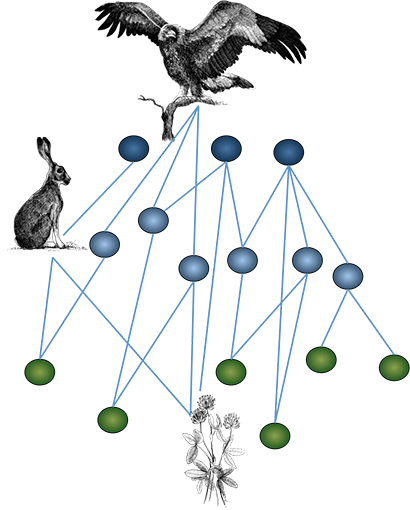
\includegraphics[width=.3\textwidth]{\figeco/ecological-networks-and-community-ecology50}
    $$
   \end{tabular}
   &
   \begin{tabular}{p{.45\textwidth}}
    $$
    \includegraphics[width=.45\textwidth]{\figeco/FaR12-Nature-Fig3a}
    $$
   \end{tabular}
  \end{tabular}
}

%==================================================================
\frame{\frametitle{Two different situations}

  \paragraph{Interactions are not-observed.} 
  \begin{itemize}
   \item Species abundance or presence/absence data (co-occurrence 'networks')
   \item Deep sequencing, metagenomics
  \end{itemize}
  \ra Reconstruct the 'interaction' network \ra \emphase{Lecture 1}

  \bigskip \bigskip 
  \paragraph{Interactions are observed.} 
  \begin{itemize}
   \item Interaction networks, contact networks
   \item Trophic networks, plant-pollinators networks
  \end{itemize}
  \ra Understand the organization/functioning  of the network \ra \emphase{Lecture 2}


}

%==================================================================
\frame{\frametitle{Network reconstruction}

  \paragraph{Generic problem:} $n$ sites, $p$ species, $d$ covariates
  
\pause \hspace{-0.06\textwidth}
\begin{tabular}{c|c|l}
  \onslide+<2->{\paragraph{Abundances:} $Y = n \times p$}
  & 
  \onslide+<3->{\paragraph{Covariates:} $X = n \times d$}
  & 
  \onslide+<4>{\paragraph{Network:} $G = p \times p$ }
  \\
  \hspace{-.02\textwidth} 
  \begin{tabular}{p{.28\textwidth}}
    \onslide+<2->{\begin{tabular}{rrr}
      {\sl Hi.pl} & {\sl An.lu} & {\sl Me.ae} 
      %\footnote{{\sl Hi.pl}: Long rough dab, {\sl An.lu}: Atlantic wolffish, {\sl Me.ae}: Haddock} 
      \\ 
%       Dab & Wolffish & Haddock \\ 
      \hline
      31  &   0  & 108 \\
       4  &   0  & 110 \\
      27  &   0  & 788 \\
      13  &   0  & 295 \\
      23  &   0  &  13 \\
      20  &   0  &  97 \\
      \vdots & \vdots & \vdots 
    \end{tabular}} 
  \end{tabular}
  & 
  \begin{tabular}{p{.3\textwidth}}
    \onslide+<3->{\begin{tabular}{rrr}
      Lat. & Long. & Depth \\ \hline
      71.10 & 22.43 & 349 \\
      71.32 & 23.68 & 382 \\
      71.60 & 24.90 & 294 \\
      71.27 & 25.88 & 304 \\
      71.52 & 28.12 & 384 \\
      71.48 & 29.10 & 344 \\
      \vdots & \vdots & \vdots 
    \end{tabular}} 
  \end{tabular}
  & 
  \hspace{-.02\textwidth} \pause
  \begin{tabular}{p{.3\textwidth}}
    \onslide+<4>{\hspace{-.1\textwidth} 
      \begin{tabular}{c}
        \includegraphics[width=.35\textwidth]{\figCMR/network_BarentsFish_Gfull_full60edges}
      \end{tabular}}
  \end{tabular}
\end{tabular}
  
\begin{itemize}
\item sites could be dates, positions along a gradient
\item 'abundances' could be presence/absence, read counts, etc..
\end{itemize}

\bigskip 
\onslide+<4>{\paragraph{Goal:} infer $G$ based on $X$ and $Y$.}
}

%==================================================================
\frame{\frametitle{Not an easy task}

  \paragraph{A huge search space:}
  $$
  \includegraphics[trim=50 50 0 75, height=.5\textheight, clip]{\fignet/NbGraphs}
  $$
  Number of \textcolor{darkgreen}{undirected graphs} ($2^{p(p-1)/2}$), \textcolor{red}{directed acyclic graphs} (no close form), \textcolor{blue}{spanning trees} ($p^{p-2}$)
}


\section[Directed graphical models]{Directed graphical models} 
\frame{\frametitle{Outline} \tableofcontents[currentsection]}
%==================================================================
\frame{\frametitle{Graphical models} 

  \bigskip
  \paragraph{'Interaction':} 
  need for a probabilistic / statistical counterpart for this concept

  \bigskip 
  \paragraph{Translation:} 
  $$
  \text{species interactions} 
  := 
  \text{dependency structure of a set of random variables}
  $$
  
  \pause\bigskip
  \begin{tabular}{lll}
    \paragraph{Graphical models:} &
    \paragraph{Directed models.} ~ &
    \paragraph{Undirected models.} ~ \\
    \begin{tabular}{p{0.3\textwidth}} A generic \\ framework \\ \refer{Lau96,WaJ08} \end{tabular}
    & 
    \begin{tabular}{p{0.3\textwidth}}   \begin{tikzpicture}
    \node[observed] (a) at (.5*\edgeunit, 2.75*\edgeunit) {$A$};
  \node[observed] (b) at (0*\edgeunit, 2*\edgeunit) {$B$};
  \node[observed] (c) at (1*\edgeunit, 2*\edgeunit) {$C$};
  \node[observed] (d) at (0.5*\edgeunit, 1*\edgeunit) {$D$};
  \node[observed] (e) at (0*\edgeunit, 0*\edgeunit) {$E$};
  \node[observed] (f) at (1*\edgeunit, 0*\edgeunit) {$F$};

  
  \draw[arrow] (a) to (b);  \draw[arrow] (a) to (c);
  \draw[arrow] (b) to (d);  \draw[arrowbendleft] (b) to (f);
  \draw[arrow] (c) to (d);  \draw[arrow] (d) to (e);
  \draw[arrow] (d) to (f);  
  \end{tikzpicture}
 \end{tabular}
    & 
    \begin{tabular}{p{0.3\textwidth}}   \begin{tikzpicture}
  %   \node[observed] (a) at (0.75*\edgeunit, 1.5*\edgeunit) {$A$};
%   \node[observed] (b) at (0*\edgeunit, 0.75*\edgeunit) {$B$};
%   \node[observed] (c) at (0.75*\edgeunit, 0*\edgeunit) {$C$};
%   \node[observed] (d) at (1.5*\edgeunit, 0.75*\edgeunit) {$D$};
%   \node[observed] (e) at (2.25*\edgeunit, 0*\edgeunit) {$E$};
%   \node[observed] (f) at (3*\edgeunit, 0.75*\edgeunit) {$F$};
%   \node[observed] (g) at (2.25*\edgeunit, 1.5*\edgeunit) {$G$};

  \node[observed] (a) at (.5*\edgeunit, 3*\edgeunit) {$A$};
  \node[observed] (b) at (0*\edgeunit, 2.25*\edgeunit) {$B$};
  \node[observed] (c) at (1*\edgeunit, 2.25*\edgeunit) {$C$};
  \node[observed] (d) at (0.5*\edgeunit, 1.5*\edgeunit) {$D$};
  \node[observed] (e) at (0*\edgeunit, .75*\edgeunit) {$E$};
  \node[observed] (f) at (1*\edgeunit, .75*\edgeunit) {$F$};
  \node[observed] (g) at (.5*\edgeunit, 0*\edgeunit) {$G$};

  
  \draw[edge] (a) to (b);  \draw[edge] (a) to (c);  \draw[edge] (a) to (d);
  \draw[edge] (b) to (c);  \draw[edge] (b) to (d);  \draw[edge] (c) to (d);
  \draw[edge] (d) to (e);  \draw[edge] (d) to (f);  \draw[edge] (e) to (f);
  \draw[edge] (f) to (g);  
  \end{tikzpicture}

 \end{tabular}
    \end{tabular}
  }

%==================================================================
\subsection*{Directed graphical models}
%==================================================================
\frame{\frametitle{Directed graphs = Bayesian networks}

  \paragraph{Definition.} Let $D$ be a {\sl directed acyclic graph} (\emphase{DAG}), the distribution $p$ is said to factorize in $D$ iff
  $$
  p(x_1, \dots x_n) = \prod_{i=1}^n p(x_i \mid x_{pa_D(i)})
  $$
  where $pa_D(i)$ stands for the set of parents of $i$ in $D$.

  \bigskip \pause
  \begin{tabular}{cc}
    \begin{tabular}{c}
    $  \begin{tikzpicture}
    \node[observed] (a) at (.5*\edgeunit, 2.75*\edgeunit) {$A$};
  \node[observed] (b) at (0*\edgeunit, 2*\edgeunit) {$B$};
  \node[observed] (c) at (1*\edgeunit, 2*\edgeunit) {$C$};
  \node[observed] (d) at (0.5*\edgeunit, 1*\edgeunit) {$D$};
  \node[observed] (e) at (0*\edgeunit, 0*\edgeunit) {$E$};
  \node[observed] (f) at (1*\edgeunit, 0*\edgeunit) {$F$};

  
  \draw[arrow] (a) to (b);  \draw[arrow] (a) to (c);
  \draw[arrow] (b) to (d);  \draw[arrowbendleft] (b) to (f);
  \draw[arrow] (c) to (d);  \draw[arrow] (d) to (e);
  \draw[arrow] (d) to (f);  
  \end{tikzpicture}
$
    \end{tabular}
    &
    \begin{tabular}{p{.7\textwidth}}
      \begin{eqnarray*}
        pa_D(A) = \emptyset, & & pa_D(D) = \{B, C\}, \qquad \dots  \\
        \\
        p(a, \dots f) & = 
        & p(a) \; p(b \mid a) \; p(c \mid a) \\
        & & p(d \mid b, c) \; p(e \mid d) \\
        & & p(f \mid b, d)
        \end{eqnarray*}
    \end{tabular}
  \end{tabular}
  
  \bigskip
  See \refer{SWA17} for an introduction in ecology
}


%==================================================================
\frame{\frametitle{A simple (interesting) example}

  Consider $D =$
  $$
    \begin{tikzpicture}
  \node[observed] (x) at (0*\edgeunit, 0*\edgeunit) {$X$};
  \node[observed] (y) at (1*\edgeunit, 0*\edgeunit) {$Y$};
  \node[observed] (z) at (2*\edgeunit, 0*\edgeunit) {$Z$};
  
  \draw[arrow] (x) to (y);  \draw[arrow] (y) to (z);
  \end{tikzpicture}

  $$
  $p(x, y, z)$ is faithful to $D$ iff
  $$
  p(x, y, z) = p(x) \; p(y \mid x) \; p(z \mid y) 
  $$ \pause
  But
  \begin{align*}
   p(x) \; p(y \mid x) \; p(z \mid y) 
%    & = p(x) \; \frac{p(x, y)}{p(x)} \; \frac{p(y, z)}{p(y)} \\
%    & = \frac{p(x, y)}{p(y)} \; \frac{p(y, z)}{p(z)} \; p(z) \\
   & = p(x \mid y) \; p(y \mid z) \; p(z) 
  \end{align*}
  so $p$ is also faithful to $D' =$
  $$
    \begin{tikzpicture}
  \node[observed] (x) at (0*\edgeunit, 0*\edgeunit) {$X$};
  \node[observed] (y) at (1*\edgeunit, 0*\edgeunit) {$Y$};
  \node[observed] (z) at (2*\edgeunit, 0*\edgeunit) {$Z$};
  
  \draw[arrow] (z) to (y);  \draw[arrow] (y) to (x);
  \end{tikzpicture}
 
  $$
  \pause and to $D'' =$
  $$
    \begin{tikzpicture}
  \node[observed] (x) at (0*\edgeunit, 0*\edgeunit) {$X$};
  \node[observed] (y) at (1*\edgeunit, 0*\edgeunit) {$Y$};
  \node[observed] (z) at (2*\edgeunit, 0*\edgeunit) {$Z$};
  
  \draw[arrow] (y) to (z);  \draw[arrow] (y) to (x);
  \end{tikzpicture}

  $$
  \bigskip 
  \pause but not to $D''' =$
  $$
    \begin{tikzpicture}
  \node[observed] (x) at (0*\edgeunit, 0*\edgeunit) {$X$};
  \node[observed] (y) at (1*\edgeunit, 0*\edgeunit) {$Y$};
  \node[observed] (z) at (2*\edgeunit, 0*\edgeunit) {$Z$};
  
  \draw[arrow] (x) to (y);  \draw[arrow] (z) to (y);
  \end{tikzpicture}

  $$  
}
  
%====================================================================
\frame{\frametitle{Interpretability?}

  \paragraph{Theorem \refer{Pea09}.} 
  Two DAGs are Markov equivalent (i.e. induce the same conditional dependences and independences) if they have the \emphase{same skeleton} (i.e. the same undirected edges) and the \emphase{same V-structures}.

  \bigskip \bigskip \pause
  \paragraph{Example.}
  \begin{center}  
  \begin{tabular}{c|cc|cc}
  $D$ &
  \multicolumn{2}{c|}{Equivalent to $D$} &
  \multicolumn{2}{c}{Not equivalent to $D$} \\
  (\textcolor{red}{V-stuctures}) & & & & \\ 
%   & & & & \\ \hline & & & & \\ 
  \hline
  $  \begin{tikzpicture}
    \node[observed] (a) at (.5*\edgeunit, 2.75*\edgeunit) {$A$};
  \node[observed] (b) at (0*\edgeunit, 2*\edgeunit) {$B$};
  \node[observed] (c) at (1*\edgeunit, 2*\edgeunit) {$C$};
  \node[observed] (d) at (0.5*\edgeunit, 1*\edgeunit) {$D$};
  \node[observed] (e) at (0*\edgeunit, 0*\edgeunit) {$E$};
  \node[observed] (f) at (1*\edgeunit, 0*\edgeunit) {$F$};


  \draw[arrow] (a) to (b);  \draw[arrow] (a) to (c);
  \draw[arrowred] (b) to (d);  \draw[arrowbendleft] (b) to (f);
  \draw[arrowred] (c) to (d);  \draw[arrow] (d) to (e);
  \draw[arrow] (d) to (f);  
  \end{tikzpicture}
$ \pause &
  $  \begin{tikzpicture}
    \node[observed] (a) at (.5*\edgeunit, 2.75*\edgeunit) {$A$};
  \node[observed] (b) at (0*\edgeunit, 2*\edgeunit) {$B$};
  \node[observed] (c) at (1*\edgeunit, 2*\edgeunit) {$C$};
  \node[observed] (d) at (0.5*\edgeunit, 1*\edgeunit) {$D$};
  \node[observed] (e) at (0*\edgeunit, 0*\edgeunit) {$E$};
  \node[observed] (f) at (1*\edgeunit, 0*\edgeunit) {$F$};


  \draw[arrowblue] (b) to (a);  \draw[arrow] (a) to (c);
  \draw[arrow] (b) to (d);  \draw[arrowbendleft] (b) to (f);
  \draw[arrow] (c) to (d);  \draw[arrow] (d) to (e);
  \draw[arrow] (d) to (f);  
  \end{tikzpicture}
$ &
  $  \begin{tikzpicture}
    \node[observed] (a) at (.5*\edgeunit, 2.75*\edgeunit) {$A$};
  \node[observed] (b) at (0*\edgeunit, 2*\edgeunit) {$B$};
  \node[observed] (c) at (1*\edgeunit, 2*\edgeunit) {$C$};
  \node[observed] (d) at (0.5*\edgeunit, 1*\edgeunit) {$D$};
  \node[observed] (e) at (0*\edgeunit, 0*\edgeunit) {$E$};
  \node[observed] (f) at (1*\edgeunit, 0*\edgeunit) {$F$};

  
  \draw[arrow] (a) to (b);  \draw[arrowblue] (c) to (a);
  \draw[arrow] (b) to (d);  \draw[arrowbendleft] (b) to (f);
  \draw[arrow] (c) to (d);  \draw[arrow] (d) to (e);
  \draw[arrow] (d) to (f);  
  \end{tikzpicture}
$ \pause &
  $  \begin{tikzpicture}
    \node[observed] (a) at (.5*\edgeunit, 2.75*\edgeunit) {$A$};
  \node[observed] (b) at (0*\edgeunit, 2*\edgeunit) {$B$};
  \node[observed] (c) at (1*\edgeunit, 2*\edgeunit) {$C$};
  \node[observed] (d) at (0.5*\edgeunit, 1*\edgeunit) {$D$};
  \node[observed] (e) at (0*\edgeunit, 0*\edgeunit) {$E$};
  \node[observed] (f) at (1*\edgeunit, 0*\edgeunit) {$F$};

  
  \draw[arrowred] (b) to (a);  \draw[arrowred] (c) to (a);
  \draw[arrow] (b) to (d);  \draw[arrowbendleft] (b) to (f);
  \draw[arrow] (c) to (d);  \draw[arrow] (d) to (e);
  \draw[arrow] (d) to (f);  
  \end{tikzpicture}
$ &
  $  \begin{tikzpicture}
    \node[observed] (a) at (.5*\edgeunit, 2.75*\edgeunit) {$A$};
  \node[observed] (b) at (0*\edgeunit, 2*\edgeunit) {$B$};
  \node[observed] (c) at (1*\edgeunit, 2*\edgeunit) {$C$};
  \node[observed] (d) at (0.5*\edgeunit, 1*\edgeunit) {$D$};
  \node[observed] (e) at (0*\edgeunit, 0*\edgeunit) {$E$};
  \node[observed] (f) at (1*\edgeunit, 0*\edgeunit) {$F$};

  
  \draw[arrow] (a) to (b);  \draw[arrow] (a) to (c);
  \draw[arrowred] (b) to (d);  \draw[arrowbendleft] (b) to (f);
  \draw[arrow] (c) to (d);  \draw[arrowred] (e) to (d);
  \draw[arrow] (d) to (f);  
  \end{tikzpicture}
$ 
  \end{tabular}
  \end{center}
  (Not speaking of possibly missing nodes)
}

%==================================================================
\frame{\frametitle{Infering directed network}

  \paragraph{Directed networks are desirable} because of interpretability but
  \begin{itemize}
   \item Visiting the space of DAGs is a hard task \refer{NPK11}
   \item Most of the time $p(x, \dots, x_n)$ is not enough to retrieve the edge orientations
   \item Many DAGs can be consistent with the observed distribution
   \item No causal interpretation of the edge orientation can be made\footnote{Causality \refer{Pea09,Pea09b} is not addressed here}
   \item All these identifiability issue arise for \emphase{known} distribution $p$, i.e. not speaking of the statistical estimation of $p$
  \end{itemize}
  
  \bigskip \bigskip \pause
  \paragraph{Still} directed network can be hoped to be inferred ... when the orientations are known.

}


\section{Temporal data} 
\frame{\frametitle{Outline} \tableofcontents[currentsection]}
% \cite{BPG18}: trop long terme

\begin{itemize}
 \item Review \& methods: \cite{FLG15}
 \item Fundamental limitations: \cite{AML17} ('all state variables are measured without any measurement noise')
 \item Actually doable? Steady-state approach: \cite{XAF17}
 \item Lotka-Volterra (simul): \cite{BeW14}
 \item Lotka-Volterra micro: \cite{SBT13}
 \item Pseudo Lotka-Volterra: \cite{AHL12}, \cite{FaR12}
 \item Presence-absence: \cite{SWA17} (data \& code: \url{https://github.com/elsander/PresenceAbsenceNetworks})
 \item Likelihood-free approach (Lotka-Volterra as an example): \cite{TRB17}
\end{itemize}



\section[Undirected graphical models]{Undirected graphical models} 
\frame{\frametitle{Outline} \tableofcontents[currentsection]}
%==================================================================
\subsection*{Undirected graphical models}
%==================================================================
\frame{\frametitle{Undirected graphs = Markov random fields}

  \paragraph{Definition.} Let $G$ be an {\sl undirected graph}, the distribution $p$ is said to factorize in $G$ iff
  $$
  p(x_1, \dots x_n) \propto \prod_{C \in \Ccal(G)} \psi_C(x_C).
  $$
  where $\Ccal(G)$ is the set of maximal cliques of $G$

  \bigskip \bigskip \pause
  \begin{tabular}{cc}
    \begin{tabular}{c}
    $  \begin{tikzpicture}
  %   \node[observed] (a) at (0.75*\edgeunit, 1.5*\edgeunit) {$A$};
%   \node[observed] (b) at (0*\edgeunit, 0.75*\edgeunit) {$B$};
%   \node[observed] (c) at (0.75*\edgeunit, 0*\edgeunit) {$C$};
%   \node[observed] (d) at (1.5*\edgeunit, 0.75*\edgeunit) {$D$};
%   \node[observed] (e) at (2.25*\edgeunit, 0*\edgeunit) {$E$};
%   \node[observed] (f) at (3*\edgeunit, 0.75*\edgeunit) {$F$};
%   \node[observed] (g) at (2.25*\edgeunit, 1.5*\edgeunit) {$G$};

  \node[observed] (a) at (.5*\edgeunit, 3*\edgeunit) {$A$};
  \node[observed] (b) at (0*\edgeunit, 2.25*\edgeunit) {$B$};
  \node[observed] (c) at (1*\edgeunit, 2.25*\edgeunit) {$C$};
  \node[observed] (d) at (0.5*\edgeunit, 1.5*\edgeunit) {$D$};
  \node[observed] (e) at (0*\edgeunit, .75*\edgeunit) {$E$};
  \node[observed] (f) at (1*\edgeunit, .75*\edgeunit) {$F$};
  \node[observed] (g) at (.5*\edgeunit, 0*\edgeunit) {$G$};

  
  \draw[edge] (a) to (b);  \draw[edge] (a) to (c);  \draw[edge] (a) to (d);
  \draw[edge] (b) to (c);  \draw[edge] (b) to (d);  \draw[edge] (c) to (d);
  \draw[edge] (d) to (e);  \draw[edge] (d) to (f);  \draw[edge] (e) to (f);
  \draw[edge] (f) to (g);  
  \end{tikzpicture}

$
    \end{tabular}
    &
    \begin{tabular}{p{.7\textwidth}}
      \begin{eqnarray*}
%         p(a, \dots g) & \propto 
%         & \psi_1(a, b, c) \; \psi_2(a, b, d) \; \psi_3(a, c, d) \; \psi_4(b, c, d) \\
%         & & \psi_5(d, e, f) \; \psi_6(f, g) \\\pause
%       \text{but also} \qquad \\
        p(a, \dots g) & \propto 
        & \psi_1(a, b, c, d) \\
        & & \psi_2(d, e, f) \; \psi_3(f, g) 
      \end{eqnarray*}
%       \ra Only consider \emphase{maximal} cliques
    \end{tabular}
  \end{tabular}
}

%====================================================================
\frame{\frametitle{Conditional independence}

  \paragraph{Property.} If $p(x) > 0$, 
  $$
  \text{separation} \qquad \Leftrightarrow \qquad \text{conditional independence}
  $$

  \bigskip \pause
  \begin{tabular}{ccc}
    \hspace{.2\textwidth} 
    &
    \begin{tabular}{c}
    $  \begin{tikzpicture}
  %   \node[observed] (a) at (0.75*\edgeunit, 1.5*\edgeunit) {$A$};
%   \node[observed] (b) at (0*\edgeunit, 0.75*\edgeunit) {$B$};
%   \node[observed] (c) at (0.75*\edgeunit, 0*\edgeunit) {$C$};
%   \node[observed] (d) at (1.5*\edgeunit, 0.75*\edgeunit) {$D$};
%   \node[observed] (e) at (2.25*\edgeunit, 0*\edgeunit) {$E$};
%   \node[observed] (f) at (3*\edgeunit, 0.75*\edgeunit) {$F$};
%   \node[observed] (g) at (2.25*\edgeunit, 1.5*\edgeunit) {$G$};

  \node[observed] (a) at (.5*\edgeunit, 3*\edgeunit) {$A$};
  \node[observed] (b) at (0*\edgeunit, 2.25*\edgeunit) {$B$};
  \node[observed] (c) at (1*\edgeunit, 2.25*\edgeunit) {$C$};
  \node[observed] (d) at (0.5*\edgeunit, 1.5*\edgeunit) {$D$};
  \node[observed] (e) at (0*\edgeunit, .75*\edgeunit) {$E$};
  \node[observed] (f) at (1*\edgeunit, .75*\edgeunit) {$F$};
  \node[observed] (g) at (.5*\edgeunit, 0*\edgeunit) {$G$};

  
  \draw[edge] (a) to (b);  \draw[edge] (a) to (c);  \draw[edge] (a) to (d);
  \draw[edge] (b) to (c);  \draw[edge] (b) to (d);  \draw[edge] (c) to (d);
  \draw[edge] (d) to (e);  \draw[edge] (d) to (f);  \draw[edge] (e) to (f);
  \draw[edge] (f) to (g);  
  \end{tikzpicture}

$
    \end{tabular}
    &
    \begin{tabular}{p{.7\textwidth}}
    \begin{itemize}
     \item $A \not\independent B$ \\ ~
     \item $A \not\independent D \mid B$ \\ ~
     \item $A \independent D \mid \{B, C\}$ \\ ~
     \item $\{A, B, C\} \independent \{E, F, G\} \mid D$ \\ ~
     \item $\{B, C\} \independent \{E, F\} \mid D$ \\ ~
    \end{itemize}
    \end{tabular}
  \end{tabular}

  \bigskip
  \ra Inferring $G$ = Inferring conditional independences
}
  
%====================================================================
\subsection*{Missing actors}
%====================================================================
\frame{\frametitle{Missing 'actors'}

  \paragraph{Incomplete observations.} Most of the time, not all actors (species, environmental covariate, ...) are observed
  
  \bigskip \bigskip 
  \paragraph{Missing variable = marginalisation.} 
  \begin{center}
  \begin{tabular}{ccccc}
    $B \independent C \mid A$ & & $A$ missing & & $B \not\independent C$ \\
    \begin{tabular}{c}
    $  \begin{tikzpicture}
    \node[observed] (a) at (.5*\edgeunit, 0.75*\edgeunit) {$A$};
  \node[observed] (b) at (0*\edgeunit, 0*\edgeunit) {$B$};
  \node[observed] (c) at (1*\edgeunit, 0*\edgeunit) {$C$};

  
  \draw[edge] (a) to (b);  \draw[edge] (a) to (c);
  \end{tikzpicture}
$
    \end{tabular}
    & \qquad \qquad &
    \begin{tabular}{c}
    $  \begin{tikzpicture}
    \node[eliminated] (a) at (.5*\edgeunit, 0.75*\edgeunit) {$A$};
  \node[observed] (b) at (0*\edgeunit, 0*\edgeunit) {$B$};
  \node[observed] (c) at (1*\edgeunit, 0*\edgeunit) {$C$};

  
  \draw[lightedge] (a) to (b);  \draw[lightedge] (a) to (c);
  \end{tikzpicture}
$
    \end{tabular}
    & \qquad \qquad &
    \begin{tabular}{c}
    $  \begin{tikzpicture}
    \node[eliminated] (a) at (.5*\edgeunit, 0.75*\edgeunit) {$A$};
  \node[observed] (b) at (0*\edgeunit, 0*\edgeunit) {$B$};
  \node[observed] (c) at (1*\edgeunit, 0*\edgeunit) {$C$};

  
  \draw[edge] (b) to (c);
  \end{tikzpicture}
$
    \end{tabular}
  \end{tabular}
  \end{center}
  
  \bigskip
  \paragraph{Indeed:}
  $$
  p(a, b, c) = p(a) p(b \mid a) p(c \mid a)
  $$
  but $A$ is not observed, so only $p(b, c)$ can be considered:
  $$
  p(b, c) = \sum_a p(a, b, c) = \sum_a p(\emphase{a}) p(b \mid \emphase{a}) p(c \mid \emphase{a}) \neq p(b) p(c)
  $$
}

%====================================================================
\frame{\frametitle{'Spurious' edges}

  Possibly dramatic effect on the observable dependency structure:
  \begin{center}
  \begin{tabular}{ccccc}
    'Truth' && $C$ missing && $D$ missing \\
    \begin{tabular}{c}
    $  \begin{tikzpicture}
  %   \node[observed] (a) at (0.75*\edgeunit, 1.5*\edgeunit) {$A$};
%   \node[observed] (b) at (0*\edgeunit, 0.75*\edgeunit) {$B$};
%   \node[observed] (c) at (0.75*\edgeunit, 0*\edgeunit) {$C$};
%   \node[observed] (d) at (1.5*\edgeunit, 0.75*\edgeunit) {$D$};
%   \node[observed] (e) at (2.25*\edgeunit, 0*\edgeunit) {$E$};
%   \node[observed] (f) at (3*\edgeunit, 0.75*\edgeunit) {$F$};
%   \node[observed] (g) at (2.25*\edgeunit, 1.5*\edgeunit) {$G$};

  \node[observed] (a) at (.5*\edgeunit, 3*\edgeunit) {$A$};
  \node[observed] (b) at (0*\edgeunit, 2.25*\edgeunit) {$B$};
  \node[observed] (c) at (1*\edgeunit, 2.25*\edgeunit) {$C$};
  \node[observed] (d) at (0.5*\edgeunit, 1.5*\edgeunit) {$D$};
  \node[observed] (e) at (0*\edgeunit, .75*\edgeunit) {$E$};
  \node[observed] (f) at (1*\edgeunit, .75*\edgeunit) {$F$};
  \node[observed] (g) at (.5*\edgeunit, 0*\edgeunit) {$G$};

  
  \draw[edge] (a) to (b);  \draw[edge] (a) to (c);  \draw[edge] (a) to (d);
  \draw[edge] (b) to (c);  \draw[edge] (b) to (d);  \draw[edge] (c) to (d);
  \draw[edge] (d) to (e);  \draw[edge] (d) to (f);  \draw[edge] (e) to (f);
  \draw[edge] (f) to (g);  
  \end{tikzpicture}

$
    \end{tabular}
    & \qquad \qquad &
    \begin{tabular}{c}
    $  \begin{tikzpicture}
  %   \node[observed] (a) at (0.75*\edgeunit, 1.5*\edgeunit) {$A$};
%   \node[observed] (b) at (0*\edgeunit, 0.75*\edgeunit) {$B$};
%   \node[observed] (c) at (0.75*\edgeunit, 0*\edgeunit) {$C$};
%   \node[observed] (d) at (1.5*\edgeunit, 0.75*\edgeunit) {$D$};
%   \node[observed] (e) at (2.25*\edgeunit, 0*\edgeunit) {$E$};
%   \node[observed] (f) at (3*\edgeunit, 0.75*\edgeunit) {$F$};
%   \node[observed] (g) at (2.25*\edgeunit, 1.5*\edgeunit) {$G$};

  \node[observed] (a) at (.5*\edgeunit, 3*\edgeunit) {$A$};
  \node[observed] (b) at (0*\edgeunit, 2.25*\edgeunit) {$B$};
  \node[eliminated] (c) at (1*\edgeunit, 2.25*\edgeunit) {$C$};
  \node[observed] (d) at (0.5*\edgeunit, 1.5*\edgeunit) {$D$};
  \node[observed] (e) at (0*\edgeunit, .75*\edgeunit) {$E$};
  \node[observed] (f) at (1*\edgeunit, .75*\edgeunit) {$F$};
  \node[observed] (g) at (.5*\edgeunit, 0*\edgeunit) {$G$};

  
  \draw[edge] (a) to (b);  \draw[lightedge] (a) to (c);  \draw[edge] (a) to (d);
  \draw[lightedge] (b) to (c);  \draw[edge] (b) to (d);  \draw[lightedge] (c) to (d);
  \draw[edge] (d) to (e);  \draw[edge] (d) to (f);  \draw[edge] (e) to (f);
  \draw[edge] (f) to (g);  
  \end{tikzpicture}
$
    \end{tabular}
    & \qquad \qquad &
    \begin{tabular}{c}
    $  \begin{tikzpicture}
  %   \node[observed] (a) at (0.75*\edgeunit, 1.5*\edgeunit) {$A$};
%   \node[observed] (b) at (0*\edgeunit, 0.75*\edgeunit) {$B$};
%   \node[observed] (c) at (0.75*\edgeunit, 0*\edgeunit) {$C$};
%   \node[observed] (d) at (1.5*\edgeunit, 0.75*\edgeunit) {$D$};
%   \node[observed] (e) at (2.25*\edgeunit, 0*\edgeunit) {$E$};
%   \node[observed] (f) at (3*\edgeunit, 0.75*\edgeunit) {$F$};
%   \node[observed] (g) at (2.25*\edgeunit, 1.5*\edgeunit) {$G$};

  \node[observed] (a) at (.5*\edgeunit, 3*\edgeunit) {$A$};
  \node[observed] (b) at (0*\edgeunit, 2.25*\edgeunit) {$B$};
  \node[observed] (c) at (1*\edgeunit, 2.25*\edgeunit) {$C$};
  \node[eliminated] (d) at (0.5*\edgeunit, 1.5*\edgeunit) {$D$};
  \node[observed] (e) at (0*\edgeunit, .75*\edgeunit) {$E$};
  \node[observed] (f) at (1*\edgeunit, .75*\edgeunit) {$F$};
  \node[observed] (g) at (.5*\edgeunit, 0*\edgeunit) {$G$};

  
  \draw[edge] (a) to (b);  \draw[edge] (a) to (c);  \draw[lightedge] (a) to (d);
  \draw[edge] (b) to (c);  \draw[lightedge] (b) to (d);  \draw[lightedge] (c) to (d);
  \draw[lightedge] (d) to (e);  \draw[lightedge] (d) to (f);  \draw[edge] (e) to (f);
  \draw[edge] (f) to (g);  

  \draw[edgered] (a) to (e);  \draw[edgered] (b) to (e);  \draw[edgebendrightred] (c) to (e);    
  \draw[edgered] (a) to (f);  \draw[edgebendleftred] (b) to (f);  \draw[edgered] (c) to (f);  
  \end{tikzpicture}
$
    \end{tabular}
  \end{tabular}
  \end{center}
  
  \bigskip
  \ra Need to account for 'all' available information to avoid 'spurious' edges

}




\section{Network inference} 
\frame{\frametitle{Outline} \tableofcontents[currentsection]}
%==================================================================
\subsection*{Latent GGM}
\frame{\frametitle{Back to ecology}

}

%==================================================================
\frame{\frametitle{Poisson log-normal model}

  \paragraph{Data:} $n$ independent sites (no spatial structure), $p$ species, 
  $$
  Y_{ij} = \text{ abundance of species $j$ in site $i$}
  $$
  
  \bigskip \pause
  \paragraph{Poisson log-normal (PLN) model \refer{AiH89}:} 
  \begin{itemize}
   \item For each site, draw independently
   $$
   Z_i \sim \Ncal_p(0, \Omega^{-1})
   $$
   \item \pause For each species in each site, draw independently (given $Z$)
   $$
   Y_{ij} \sim \Pcal(\exp(\mu_j + Z_{ij}))
   $$
  \end{itemize} \pause
  summarized as
  $$
  \{Y_i\} \text{ iid} \sim PLN(\mu, \Omega^{-1})
  $$

  \bigskip \pause
  \paragraph{Interpretation.}
  \begin{itemize}
%   \item PLN is a mixed model
  \item $\mu_j =$ mean (log-)abundance of species $j$
  \item $\Omega = $ dependency structure (encoded in the latent layer)
  \end{itemize}
}

%==================================================================
\frame{\frametitle{PLNnetworks}

  \paragraph{PLN network model.} Same model as PLN + sparsity assumption:
  $$
  \{Y_i\} \text{ iid} \sim PLN(\mu, \Omega)
  \qquad \qquad + \emphase{\Omega \text{ sparse}}
  $$
  
  \bigskip \bigskip \pause
  \paragraph{Inference algorithm.} Variational EM + sparsity inducing norm \refer{CMR18,CMR19}:
  $$
  \max_{\mu, \Omega} \widetilde{\log p}(Y; \mu, \Omega) - \lambda \sum_{j < k} |\omega_{jk}|
  $$
  \ra Alternate convex problems \\
  \ra Fast solution ({\tt PLNmodels} R package)
  
  \bigskip
  \begin{itemize}
   \item Resampling (StARS \refer{LRW10}) is highly recommended for robustness
  \end{itemize}
}

%==================================================================
\frame{\frametitle{Modeling limitation}

  \paragraph{All latent (GGM) models} infer the dependency struture of the latent $Z$, not of the observed abundances $Y$
  
  \bigskip \bigskip 
  \renewcommand{\nodesize}{2em}
  \begin{overprint}
    \onslide<2>
    $$
    \begin{array}{ccc}
    p(Z, Y) & & p(Y) \\ ~\\
      \begin{tikzpicture}[scale=.8]
  \node[hidden] (Z1) at ( 0.95*\edgeunit,  0.31*\edgeunit) {$Z_1$};
  \node[hidden] (Z2) at (-0.00*\edgeunit,  1.00*\edgeunit) {$Z_2$};
  \node[hidden] (Z3) at (-0.95*\edgeunit,  0.31*\edgeunit) {$Z_3$};
  \node[hidden] (Z4) at (-0.59*\edgeunit, -0.81*\edgeunit) {$Z_4$};
  \node[hidden] (Z5) at ( 0.59*\edgeunit, -0.81*\edgeunit) {$Z_5$};
  
  \draw[edge] (Z1) to (Z5);  \draw[edge] (Z2) to (Z3);  
  \draw[edge] (Z2) to (Z4);  \draw[edge] (Z3) to (Z4); 

  \node[observed] (Y1) at ( 1.05*\edgeunit, -0.39*\edgeunit) {$Y_1$};
  \node[observed] (Y2) at (-0.00*\edgeunit,  0.30*\edgeunit) {$Y_2$};
  \node[observed] (Y3) at (-1.05*\edgeunit, -0.39*\edgeunit) {$Y_3$};
  \node[observed] (Y4) at (-0.59*\edgeunit, -1.51*\edgeunit) {$Y_4$};
  \node[observed] (Y5) at ( 0.59*\edgeunit, -1.51*\edgeunit) {$Y_5$};
  
  \draw[arrow] (Z1) to (Y1); 
  \draw[arrow] (Z2) to (Y2);
  \draw[arrow] (Z3) to (Y3);
  \draw[arrow] (Z4) to (Y4);
  \draw[arrow] (Z5) to (Y5);
  \end{tikzpicture}

    & \qquad \qquad &
      \begin{tikzpicture}[scale=.8]
  \node[observed] (Y1) at ( 0.95*\edgeunit,  0.31*\edgeunit) {$Y_1$};
  \node[observed] (Y2) at (-0.00*\edgeunit,  1.00*\edgeunit) {$Y_2$};
  \node[observed] (Y3) at (-0.95*\edgeunit,  0.31*\edgeunit) {$Y_3$};
  \node[observed] (Y4) at (-0.59*\edgeunit, -0.81*\edgeunit) {$Y_4$};
  \node[observed] (Y5) at ( 0.59*\edgeunit, -0.81*\edgeunit) {$Y_5$};
  \node[empty] (YY) at ( 0.59*\edgeunit, -1.51*\edgeunit) {};

  \draw[edge] (Y1) to (Y5);  \draw[edge] (Y2) to (Y3);  
  \draw[edge] (Y2) to (Y4);  \draw[edge] (Y3) to (Y4);  
  
  \end{tikzpicture}

    \end{array}
    $$
    \onslide<3>
    $$
    \begin{array}{ccc}
    p(Z, Y) & & p(Y) \\ ~\\
      \begin{tikzpicture}[scale=.8]
    \node[hidden] (Z1) at ( 0.95*\edgeunit,  0.31*\edgeunit) {$Z_1$};
    \node[hidden] (Z2) at (-0.00*\edgeunit,  1.00*\edgeunit) {$Z_2$};
    \node[hidden] (Z3) at (-0.95*\edgeunit,  0.31*\edgeunit) {$Z_3$};
    \node[hidden] (Z4) at (-0.59*\edgeunit, -0.81*\edgeunit) {$Z_4$};
    \node[hidden] (Z5) at ( 0.59*\edgeunit, -0.81*\edgeunit) {$Z_5$};
    
    \draw[edge] (Z1) to (Z2);  \draw[edge] (Z1) to (Z4);  
    \draw[edge] (Z1) to (Z5);  \draw[edge] (Z2) to (Z3);  
    \draw[edge] (Z2) to (Z4);  \draw[edge] (Z3) to (Z4); 

    \node[observed] (Y1) at ( 1.05*\edgeunit, -0.39*\edgeunit) {$Y_1$};
    \node[observed] (Y2) at (-0.00*\edgeunit,  0.30*\edgeunit) {$Y_2$};
    \node[observed] (Y3) at (-1.05*\edgeunit, -0.39*\edgeunit) {$Y_3$};
    \node[observed] (Y4) at (-0.59*\edgeunit, -1.51*\edgeunit) {$Y_4$};
    \node[observed] (Y5) at ( 0.59*\edgeunit, -1.51*\edgeunit) {$Y_5$};

    \draw[arrow] (Z1) to (Y1); 
    \draw[arrow] (Z2) to (Y2);
    \draw[arrow] (Z3) to (Y3);
    \draw[arrow] (Z4) to (Y4);
    \draw[arrow] (Z5) to (Y5);
  \end{tikzpicture}

    & \qquad \qquad &
      \begin{tikzpicture}[scale=.8]
  \node[observed] (Y1) at ( 0.95*\edgeunit,  0.31*\edgeunit) {$Y_1$};
  \node[observed] (Y2) at (-0.00*\edgeunit,  1.00*\edgeunit) {$Y_2$};
  \node[observed] (Y3) at (-0.95*\edgeunit,  0.31*\edgeunit) {$Y_3$};
  \node[observed] (Y4) at (-0.59*\edgeunit, -0.81*\edgeunit) {$Y_4$};
  \node[observed] (Y5) at ( 0.59*\edgeunit, -0.81*\edgeunit) {$Y_5$};
  \node[empty] (YY) at ( 0.59*\edgeunit, -1.51*\edgeunit) {};

  \draw[edge] (Y1) to (Y2);  \draw[edge] (Y1) to (Y3);  
  \draw[edge] (Y1) to (Y4);  \draw[edge] (Y1) to (Y5);  
  \draw[edge] (Y2) to (Y3);  \draw[edge] (Y2) to (Y4); 
  \draw[edge] (Y2) to (Y5);  \draw[edge] (Y3) to (Y4);  
  \draw[edge] (Y3) to (Y5);  \draw[edge] (Y4) to (Y5);  
  \end{tikzpicture}

    \end{array}
    $$
  \end{overprint}
  \renewcommand{\nodesize}{\commonnodesize}
}

%==================================================================
\frame{\frametitle{Illustration}

  \paragraph{Barents fish dataset:} $n = 89$ sites, $p = 30$ species
  
  \bigskip
  \begin{tabular}{p{.45\textwidth}p{.45\textwidth}}
    \begin{tabular}{c}
      \vspace{.04\textheight}
      Regularization path ($\lambda$) \\
      \includegraphics[width=.45\textwidth, height=.45\textheight]{\figbarents/BarentsFish_Gnull_criteria}
    \end{tabular}
    &
%     \hspace{-.1\textwidth}
    \begin{overprint}
      \onslide<2>
        \begin{tabular}{c}
          Covariance ($\widehat{\Sigma}$) \\ 
          \includegraphics[width=.4\textwidth]{\figbarents/BarentsFish_Gnull_sigma}
        \end{tabular}
      \onslide<3>
        \begin{tabular}{c}
          Precision ($\widehat{\Omega}$) \\ 
          \includegraphics[width=.4\textwidth]{\figbarents/BarentsFish_Gnull_omega}
        \end{tabular}
      \onslide<4>
        \begin{tabular}{c}
          Network ($\widehat{G}$) \\ 
          \includegraphics[width=.4\textwidth]{\figbarents/BarentsFish_Gnull_network}
        \end{tabular}
    \end{overprint}
  \end{tabular}

  {\tt PLNnetwork} R package  \refer{CMR19}: \qquad
  {\tt PLNnetwork(Y $\sim$  1)}
}

%==================================================================
\subsection*{Accounting for covariates}
\frame{\frametitle{Accounting for covariates}

  \paragraph{Aim of network inference:} determine which species are 'in direct interaction' \\
  \ra Avoid 'spurious edges'
  
  \hspace{-.05\textwidth}
  \begin{tabular}{p{.45\textwidth}p{.45\textwidth}}
    \begin{tabular}{p{.4\textwidth}}
      \onslide+<2->{
        \paragraph{Environmental variations} may jointly affect species, which do not actually interact \\
        }
      \onslide+<4->{
        \bigskip \bigskip 
        \paragraph{Introducing covariates.} ~ \\
        $x_i =$ vector of covariates for site $i$ \\
        e.g. $x_i = (\text{temperature}, \text{altitude}, ...)$
        }
    \end{tabular}
    &
%     \hspace{-.1\textwidth}
    \begin{tabular}{p{.45\textwidth}}
      \onslide+<3->{
        \includegraphics[width=.4\textwidth]{\figbarents/BarentsFish_Sigmanull_Sigmafull}
        }
    \end{tabular}
  \end{tabular}
  
  \onslide+<4->{
    Add a regression term in the PLN model:
    $$
    Y_{ij} \mid Z_{ij} \sim \Pcal(\exp(\emphase{x_i^\intercal \beta_j} + Z_{ij}))
    $$
    $\beta_j =$ vector of environmental effects on species $j$
    }

}

%====================================================================
\frame{\frametitle{Barents fish} 

  \begin{center}
  \begin{tabular}{lccc}
    & no covariate & \textcolor{blue}{temp. \& depth} & \textcolor{red}{all covariates} \\
    \hline
    \rotatebox{90}{$\qquad\quad\lambda=.20$} &
    \includegraphics[width=.22\textwidth]{\figCMR/network_BarentsFish_Gnull_full60edges} &
    \includegraphics[width=.22\textwidth]{\figCMR/network_BarentsFish_Gsel_full60edges} &
    \includegraphics[width=.22\textwidth]{\figCMR/network_BarentsFish_Gfull_full60edges} 
    \vspace{-0.05\textheight} \\ \hline
    %
    \rotatebox{90}{$\qquad\quad\lambda=.28$} &
    \includegraphics[width=.22\textwidth]{\figCMR/network_BarentsFish_Gnull_sel60edges} & \includegraphics[width=.22\textwidth]{\figCMR/network_BarentsFish_Gsel_sel60edges} &
    \includegraphics[width=.22\textwidth]{\figCMR/network_BarentsFish_Gfull_sel60edges} 
    \vspace{-0.05\textheight} \\ \hline
    %
    \rotatebox{90}{$\qquad\quad\lambda=.84$} &
    \includegraphics[width=.22\textwidth]{\figCMR/network_BarentsFish_Gnull_null60edges} &
    \includegraphics[width=.22\textwidth]{\figCMR/network_BarentsFish_Gsel_null60edges} &
    \includegraphics[width=.22\textwidth]{\figCMR/network_BarentsFish_density} 
%     \includegraphics[width=.22\textwidth]{\figCMR/network_BarentsFish_Gfull_null60edges}  
  \end{tabular}
  \end{center}

}



\section{Conclusion ?} 
\frame{\frametitle{Outline} \tableofcontents[currentsection]}
%==================================================================
\frame{\frametitle{Discussion}

  \paragraph{Network inference is} 
  \begin{itemize}
   \item Not always a very well-posed problem
   \item A difficult task because of its combinatorial dimension ('a needle in a haystack')
   \item Slightly easier for undirected networks
   \item A highly unsupervised problem (nobody knows the truth, few experimental validations exist)
  \end{itemize}
  
  \bigskip \pause
  \hspace{-.05\textwidth}
  \begin{tabular}{ll}
    \begin{tabular}{p{.55\textwidth}}
      \paragraph{Take-home-message} 
      \begin{itemize}
      \item It is not hopeless (although ...)
      \item Graphical models provide a sound mathematical framework 
      \item Reasonably simple tools (R packages) exist 
      \item Accounting for covariates has a dramatic effect on the inferred network
      \item Always ask if the question is a network question \refer{JFS16}
      \end{itemize}
    \end{tabular}
    &
    \pause
%     \hspace{-.05\textwidth}
    \begin{tabular}{p{.4\textwidth}}
      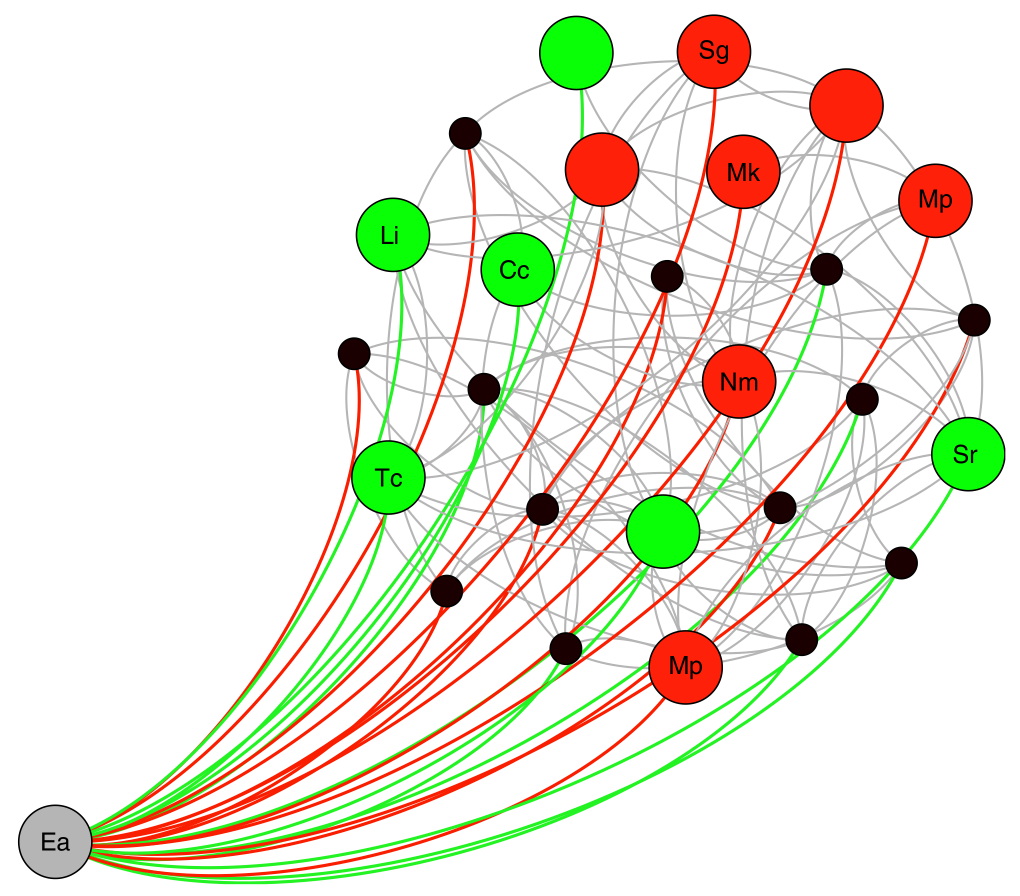
\includegraphics[width=.3\textwidth]{\fignet/JFS16-EnvirMicrobiol-Fig4}
    \end{tabular}
  \end{tabular}

}

  


%==================================================================
\backupbegin

\frame[allowframebreaks]{ \frametitle{References} 
  {\tiny
   \bibliography{/home/robin/Biblio/BibGene}
   \bibliographystyle{alpha}
  }
}

\section*{Backup} 
%====================================================================
\subsection*{Directed networks} 
%====================================================================
\frame{\frametitle{Conditional independance}

  \paragraph{Definition.} $X$ is independent of $Y$ conditional on $Z$ ($X \independent Y \mid Z$) iff
  $$
  p(x, y \mid z) = p(x \mid z) p(y \mid z)
  \qquad \Leftrightarrow \qquad 
  p(x \mid z, y) = p(x \mid z) 
  $$

  \bigskip \bigskip \pause
  \paragraph{Example.} $A \independent C \mid B$ in the 3 DAGs:
  $$
    \begin{tikzpicture}
  \node[observed] (x) at (0*\edgeunit, 0*\edgeunit) {$X$};
  \node[observed] (y) at (1*\edgeunit, 0*\edgeunit) {$Y$};
  \node[observed] (z) at (2*\edgeunit, 0*\edgeunit) {$Z$};
  
  \draw[arrow] (x) to (y);  \draw[arrow] (y) to (z);
  \end{tikzpicture}
 \qquad
    \begin{tikzpicture}
  \node[observed] (x) at (0*\edgeunit, 0*\edgeunit) {$X$};
  \node[observed] (y) at (1*\edgeunit, 0*\edgeunit) {$Y$};
  \node[observed] (z) at (2*\edgeunit, 0*\edgeunit) {$Z$};
  
  \draw[arrow] (z) to (y);  \draw[arrow] (y) to (x);
  \end{tikzpicture}
 \qquad
    \begin{tikzpicture}
  \node[observed] (x) at (0*\edgeunit, 0*\edgeunit) {$X$};
  \node[observed] (y) at (1*\edgeunit, 0*\edgeunit) {$Y$};
  \node[observed] (z) at (2*\edgeunit, 0*\edgeunit) {$Z$};
  
  \draw[arrow] (y) to (z);  \draw[arrow] (y) to (x);
  \end{tikzpicture}

  $$
  Indeed, for first one,
  $$
  p(x, z \mid y)
  = \frac{p(x, y, z)}{p(y)}
  = \frac{p(x) p(y \mid x) p(z \mid y)}{p(y)}
  = p(x \mid y) p(z \mid y)
  $$
  because $p(x) p(y \mid x) = p(y) p(x \mid y)$.
}

%====================================================================
\frame{\frametitle{V-structure}

%   \paragraph{Counter-example.} 
  In the V-structured (or 'head to head') DAG:
  $$
    \begin{tikzpicture}
  \node[observed] (x) at (0*\edgeunit, 0*\edgeunit) {$X$};
  \node[observed] (y) at (1*\edgeunit, 0*\edgeunit) {$Y$};
  \node[observed] (z) at (2*\edgeunit, 0*\edgeunit) {$Z$};
  
  \draw[arrow] (x) to (y);  \draw[arrow] (z) to (y);
  \end{tikzpicture}

  $$
  $X$ and $Z$ are \emphase{conditionally dependent} ($X \not\independent Y \mid Z$):
  \begin{align*}
  p(x, y, z) & = p(x) p(z) p(y \mid x, z) \\ ~\\
  \Rightarrow \quad
  p(x, z \mid y) & = \frac{p(x, y, z)}{p(y)}   = \frac{p(x) p(z) p(y \mid x, z)}{p(y)}  
  \end{align*}
  
  \bigskip \bigskip \pause
  \paragraph{Remark.} 
  $X$ and $Z$ are \emphase{marginally independent}:
  $$
   p(x, z)
  = \sum_y p(x) p(z) p(y \mid x, z)
  = p(x) p(z) \underset{= 1}{\underbrace{\sum_y p(y \mid x, z)}}
  $$
}


%====================================================================
\frame{\frametitle{From directed to undirected graphical models}

  \paragraph{Resolve {\sl immoralities}.} Graph {\sl moralization} (parents must be married):
  $$
  \begin{array}{ccccc}
     \begin{tikzpicture} 
    \node[observed] (a) at (0*\edgeunit, 1*\edgeunit) {$A$};
  \node[observed] (b) at (1*\edgeunit, 1*\edgeunit) {$B$};
  \node[observed] (c) at (.5*\edgeunit, 0*\edgeunit) {$C$};
  

  
  \draw[arrow] (a) to (c);  \draw[arrow] (b) to (c);
  \end{tikzpicture}
  

   & \qquad & 
     \begin{tikzpicture} 
    \node[observed] (a) at (0*\edgeunit, 1*\edgeunit) {$A$};
  \node[observed] (b) at (1*\edgeunit, 1*\edgeunit) {$B$};
  \node[observed] (c) at (.5*\edgeunit, 0*\edgeunit) {$C$};
  

  
  \draw[arrow] (a) to (c);  \draw[arrow] (b) to (c);
  \draw[dashededge] (a) to (b);
  \end{tikzpicture}
  

   & \qquad & 
     \begin{tikzpicture} 
    \node[observed] (a) at (0*\edgeunit, 1*\edgeunit) {$A$};
  \node[observed] (b) at (1*\edgeunit, 1*\edgeunit) {$B$};
  \node[observed] (c) at (.5*\edgeunit, 0*\edgeunit) {$C$};
  

  
  \draw[edge] (a) to (c);  \draw[edge] (b) to (c);
  \draw[edge] (a) to (b);
  \end{tikzpicture}
  

  \end{array}
  $$
  
  \pause
  \paragraph{Example.}
  $$
  \begin{array}{ccccc}
     \begin{tikzpicture}
    \node[observed] (a) at (.5*\edgeunit, 2.75*\edgeunit) {$A$};
  \node[observed] (b) at (0*\edgeunit, 2*\edgeunit) {$B$};
  \node[observed] (c) at (1*\edgeunit, 2*\edgeunit) {$C$};
  \node[observed] (d) at (0.5*\edgeunit, 1*\edgeunit) {$D$};
  \node[observed] (e) at (0*\edgeunit, 0*\edgeunit) {$E$};
  \node[observed] (f) at (1*\edgeunit, 0*\edgeunit) {$F$};

  
  \draw[arrow] (a) to (b);  \draw[arrow] (a) to (c);
  \draw[arrow] (b) to (d);  \draw[arrowbendleft] (b) to (f);
  \draw[arrow] (c) to (d);  \draw[arrow] (d) to (e);
  \draw[arrow] (d) to (f);  
  \end{tikzpicture}

   & \qquad & 
     \begin{tikzpicture}
    \node[observed] (a) at (.5*\edgeunit, 2.75*\edgeunit) {$A$};
  \node[observed] (b) at (0*\edgeunit, 2*\edgeunit) {$B$};
  \node[observed] (c) at (1*\edgeunit, 2*\edgeunit) {$C$};
  \node[observed] (d) at (0.5*\edgeunit, 1*\edgeunit) {$D$};
  \node[observed] (e) at (0*\edgeunit, 0*\edgeunit) {$E$};
  \node[observed] (f) at (1*\edgeunit, 0*\edgeunit) {$F$};

  
  \draw[arrow] (a) to (b);  \draw[arrow] (a) to (c);
  \draw[dashededge] (b) to (c);  
  \draw[arrow] (b) to (d);  \draw[arrowbendleft] (b) to (f);
  \draw[arrow] (c) to (d);  \draw[arrow] (d) to (e);
  \draw[arrow] (d) to (f);  
  \end{tikzpicture}

   & \qquad & 
     \begin{tikzpicture}
    \node[observed] (a) at (.5*\edgeunit, 2.75*\edgeunit) {$A$};
  \node[observed] (b) at (0*\edgeunit, 2*\edgeunit) {$B$};
  \node[observed] (c) at (1*\edgeunit, 2*\edgeunit) {$C$};
  \node[observed] (d) at (0.5*\edgeunit, 1*\edgeunit) {$D$};
  \node[observed] (e) at (0*\edgeunit, 0*\edgeunit) {$E$};
  \node[observed] (f) at (1*\edgeunit, 0*\edgeunit) {$F$};

  
  \draw[edge] (a) to (b);  \draw[edge] (a) to (c);
  \draw[edge] (b) to (c);  
  \draw[edge] (b) to (d);  \draw[edgebendleft] (b) to (f);
  \draw[edge] (c) to (d);  \draw[edge] (d) to (e);
  \draw[edge] (d) to (f);  
  \end{tikzpicture}

  \end{array}
  $$
}

%====================================================================
\subsection*{Causality}
%====================================================================
\frame{\frametitle{Causality \refer{Pea09}}

  \begin{tabular}{c|c|c}
    'Truth' & Equivalent & 'Causality' \\  
    & {based on observational data} \\  
    & & \\\hline & & \\
    \includegraphics[trim={0 15 180 0}, height=.22\textheight, clip]{\figeco/Pea09-Fig2-3}
    &
    \includegraphics[trim={0 15 0 0}, height=.21\textheight, clip]{\figeco/Pea09-Fig2-4}
    &
    \includegraphics[trim={180 15 0 0}, height=.22\textheight, clip]{\figeco/Pea09-Fig2-3}
  \end{tabular}

  \bigskip \bigskip 
  $$
  \{a \leftrightarrow b\} \qquad = \qquad \{a \leftarrow u \rightarrow b, 
  \quad \text{$u$ unobserved}\}
  $$  
}

%====================================================================
\subsection*{Dynamic networks}
% %==================================================================
% \frame{\frametitle{Lotka-Voltera interpretation}
% 
%   \begin{itemize}
%   \item Review \& methods: \refer{FLG15}
%   \item Fundamental limitations: \refer{AML17} ('all state variables are measured without any measurement noise') + \refer{Ver12}
%   \item Actually doable? Steady-state approach: \refer{XAF17}
%   \item Lotka-Volterra (simul): \refer{BeW14}
%   \item Lotka-Volterra micro: \refer{SBT13}
%   \item Pseudo Lotka-Volterra: \refer{AHL12}, \refer{FaR12}
%   \item Likelihood-free approach (Lotka-Volterra as an example): \refer{TRB17}
%   \end{itemize}
% }
% 
%====================================================================
\subsection*{Latent GGM}
%==================================================================
\frame{\frametitle{Effect of covariates}

  \paragraph{Fish species in the Fatala river \refer{Bar95}.} $n = 95$ observations, $p = 33$ fish species, $x_i =$ date and site of the observations

  \bigskip \bigskip 
  \paragraph{Inferred networks.} 
  $$
  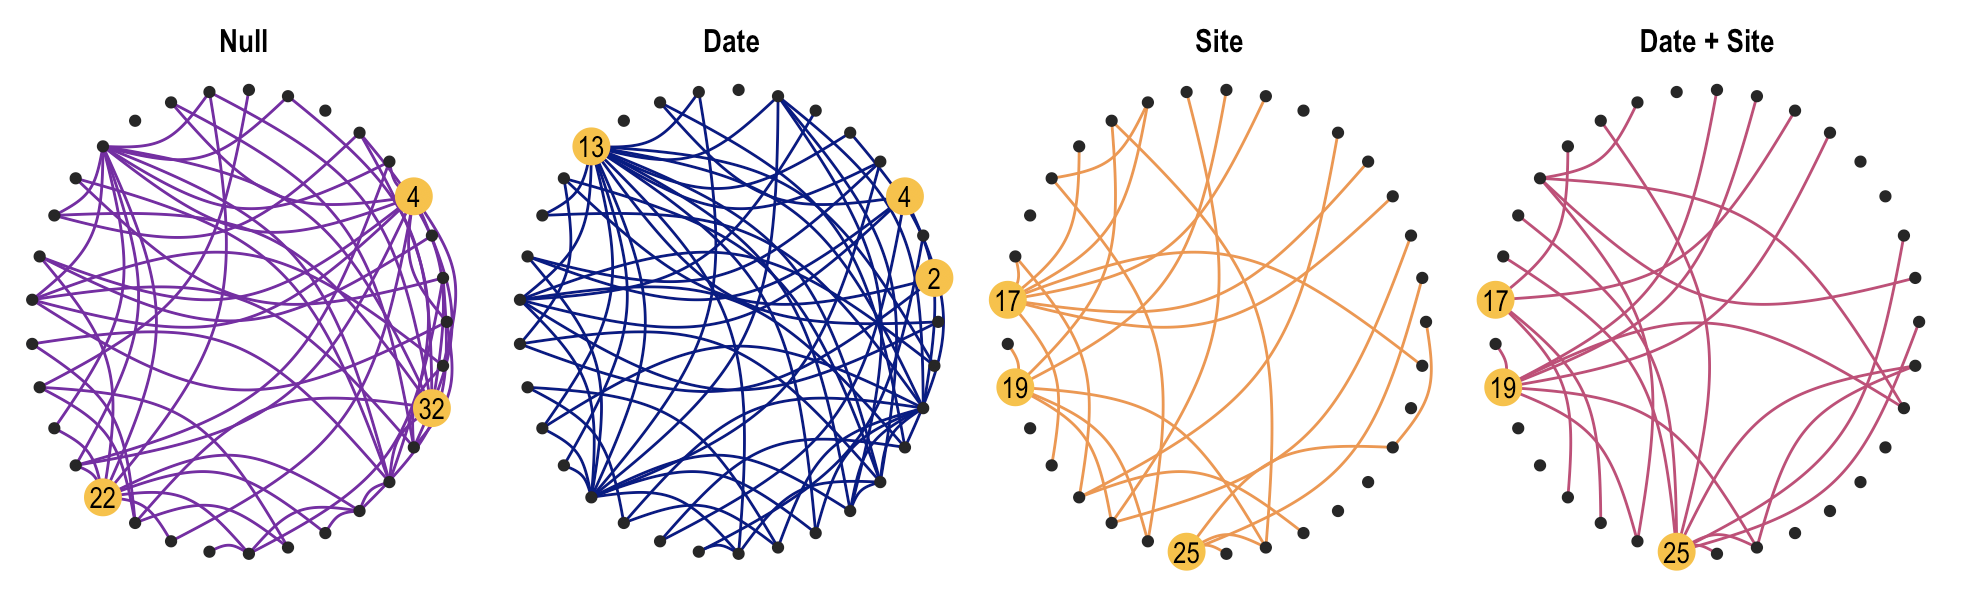
\includegraphics[width=.9\textwidth]{\fignet/MRA19-Fig8} 
  $$
  \ra Even 'key-species' change according to which covariates are taken into account.
}

\backupend

%==================================================================
%==================================================================
\end{document}
%==================================================================
%==================================================================
